%! TEX root = ../main.tex
\documentclass[main]{subfiles}

\begin{document}



\section{実装方法と使用技術}
前章で述べた本システムの主な機能を実現するための詳細な機能とそれらを実現する技術を以下に示す.図\ref{fig:techstack}

\textcircled{\scriptsize{1}}: 提案機能 \par
機能詳細:\par
(1) メインとなるフレームワークの提案:Stack Overflow Annual Developer SurveyのデータをDBに格納しAPIから取得する.\par
(2) その他ライブラリの提案:npm registryが提供するAPIから取得する.\par
(3) linter, formatterなどある程度共通認識が見込まれるライブラリの提案:採用するか否かのみをユーザに尋ね,本システム側で他のライブラリとのバージョンの互換性を検証した上でインストールツリーに組み込む.\par
使用技術:Next.js Serverless Functions, Supabase, npm registry API, React flowなど.\par

\textcircled{\scriptsize{2}},\textcircled{\scriptsize{3}},\textcircled{\scriptsize{4}}: コミュニケーション促進機能\par
機能詳細:\par
(1) ユーザの認証・認可機能:認証サーバからクライアントにJWTを発行し,公開鍵で検証することにより認証・認可する.認証後はユーザがDBに挿入・更新され,認可後は認証・認可以外のすべてのAPIが使用可能になる.\par
(2) リアルタイムチャット機能:GraphQLのsubscriptionを使用し,リアルタイムでのDBからのデータ取得を実現する.\par
(3) ユーザへのロール(役割)付与:DBにチームレコードを挿入・更新・削除するAPIなどはチームのadminユーザのみしか操作できない.\par
(4) ユーザのオンライン・オフライン表示:GraphQLのsubscriptionを使用する.\par
使用技術:Next.js Serverless Functions, Supabase, GraphQL, Hasura Engine, Auth0など.\par
\begin{figure}[h]
    \centering
    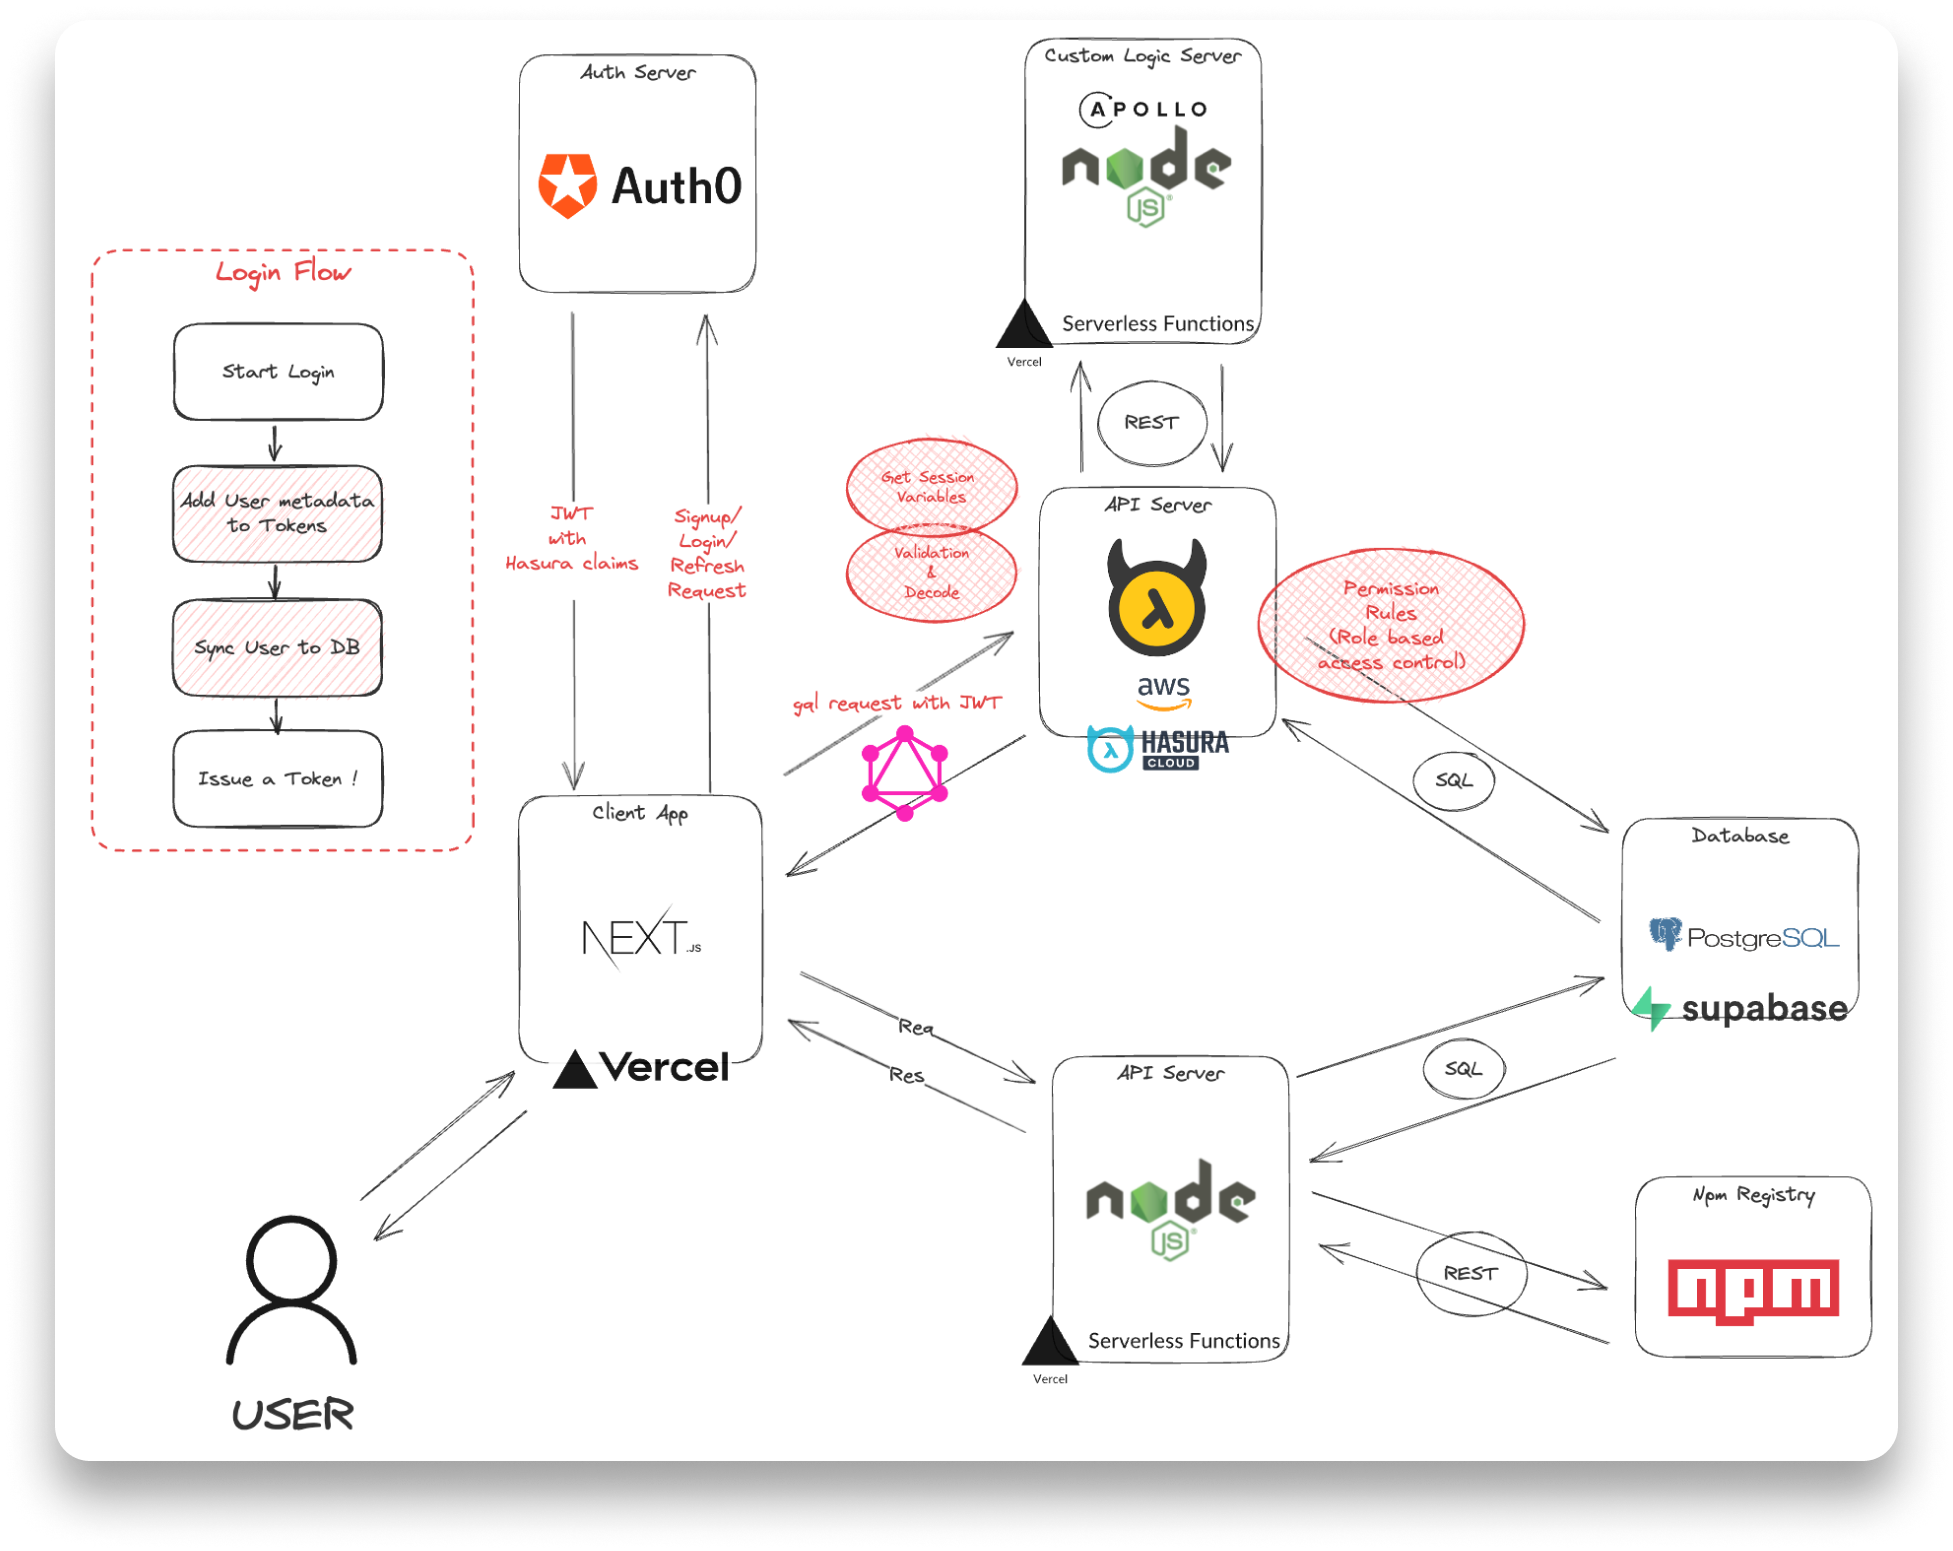
\includegraphics[keepaspectratio,width=0.5\textwidth]{../figures/techstack.png}
    \caption{技術構成図}
    \label{fig:techstack}
\end{figure}

\end{document}
